\chapter{Introduction}
\label{cha:introduction}

\section{Background}
\label{sec:Background}
Technological advances of the recent decades such as microarrays and next generation sequencing (NGS) have revolutionized our ability to interrogate the structure, function, and regulation of the genome at an unprecedented scale. It has accelerated the investigation of the effects of the genome, epigenome and transcriptome on human health, and opened the door to personalized medicine. 

Personalized medicine refers to our ability to diagnose and predict health outcomes and response to treatment based on an individual's `omic' profile, so that treatment can be taylored to optimize the individual's health outcomes. 

On top of genomic, transcriptomic and epigenomic  profiles measured on individuals, there sits a layer of `meta knowledge' about gene function, gene products and gene regulation, that is critical for interpreting the results of studies of genomics and disease. These `meta-features' can include functional annotations and previous studies. 

The purpose of this thesis is to develop high-dimensional statistical methods to integrate  genomics data with meta-features into the predictive modeling process, with the ultimate goal of improving  prediction performance and producing more interpretable results.

\section{Genomics-based prediction of disease traits}
\label{sec:Prediction}
Among the many uses of prediction of disease outcomes based on genomic data, we can distinguish between two important applications: 1) disease prognosis, namely prediction of the course of disease, and survival. We refer to genomic features predictive of these outcomes as prognostic biomarkers; 2) prediction of treatment effect, based on patients' genomics profiles, i.e., how patients they respond to a treatment. We refer to genomic features predictive of these outcomes as predictive biomarkers \citep{mandrekar2010predictive}. 

In this thesis, the focus is on predictive modeling in cancer genomics, as array- and sequencing-based assays of tumor tissue has enabled clinically actionable insights for many types of cancers. We give a brief overview of some of the predictive modeling techniques commonly used. 


\subsection{Regression}
Regression methods are widely used techniques for constructing predictive models. The most popular are linear regression for quantitative traits, logistic regression for binary and multi-category traits, and Cox's proportional hazards regression for survival traits. These regression methods rely on linear combinations of the genomic features/predictors to predict the outcome of interest. The training data consists of a response vector $\bm{Y}$ of length $n$ (for survival outcomes, it is a response matrix of dimension $n \times 2$, survival time and censoring status) and a data/design matrix $\bm{X}$ of dimension $n \times p$, where $n$ is the number of independent samples, $p$ is the number of features. The linear predictors for each of the $n$ samples are defined as $\bm{\beta}^T\bm{x}_i$, where $\bm{x}_i$ is the features for the $i^{th}$ sample, $\bm{\beta}$ is the regression coefficients to be estimated. The optimization problems for the linear and logistic cases are shown below:
\begin{align}
    &\min_{\bm{\beta}} \left\{\frac{1}{2n} \sum_{i=1}^{n} (y_i-\bm{\beta}^T\bm{x}_i)^2 \right\}, \qquad\qquad\qquad\quad\;\: \text{linear regression} \label{eq1.1} \\
    &\min_{\bm{\beta}} \left\{-\frac{1}{n} \sum_{i=1}^{n} \left[y_i\bm{\beta}^T\bm{x}_i-\ln(1+e^{\bm{\beta}^T\bm{x}_i})\right]\right\}, \qquad \text{logistic regression} \label{eq1.2}
\end{align}

We will deal in detail with the Cox's proportional hazards regression in later sections, as survival is the main type of trait this thesis will be concerned  with. Incorporation of non-linearities are possible with regression, by the inclusion of higher order and interaction terms.

There are several requirements to apply standard regression methods. First, the number of features $p$ should be less than the number of samples $n$ for the model to be able to fit. However, this is usually not the case in genomics studies because of the large number of features examined and the limits to sample size due to costs and logistics. For example, biopsies could be highly invasive depending on the location of tumors, and hence reserved for some patients. As a result, the number of samples is small to moderate at best, typical number ranging from hundreds to thousands. By contrast, the number of genomic features is often huge. There may be tens (e.g., gene expression) or even hundreds of thousands features (e.g., methylation). If there are multiple omic types, the numbers can be even larger. Therefore, genomics data are typically very high dimensional ($p>>n$). Multicollinearity between features is another serious concern. Highly correlated features should have similar regression coefficients (negatively correlated markers have opposite sign, but similar in magnitude). But in standard regression, the coefficient estimates are highly unstable when the features are highly correlated. Other concerns include marker-marker interactions, missing data. 

Regression models cannot be fit with high-dimensional data. Therefore, regularization need to be introduced. Considering a linear regression, equation \eqref{eq1.1}, the solution to it is the ordinary least square (OLS), $\hat{\bm{\beta}}=(\bm{X}^T\bm{X})^{-1}\bm{X}^T\bm{Y}$. If $\bm{X}_{n\times p}$ is high-dimensional, $p>n$, the highest rank of matrix $(\bm{X}^T\bm{X})_{p\times p}$ is $\min(p,n)=n$, so it is a singular matrix. Mathematically, there is no solution to $\bm{\beta}$. Intuitively, the model is too complex to fit because there is not enough data. Regularization is a technique to control model complexity, by shrinking the regression coefficients. Regularized regression can be written as an optimization problem of the form:
\begin{equation}
    \min_{\bm{\beta}} \left\{-\ell(\bm{\beta}) + \lambda P(\bm{\beta})\right\}, \label{eq1.3}
\end{equation}
where $\ell(\bm{\beta})$ is the log of likelihood function. $P(\bm{\beta})$ is the regularization/penalty function, which penalizes the regression coefficients and shrinks their estimates toward zero. Shrinkage stabilizes the coefficient estimates (reduces model variance) and decreases model complexity (increases bias). Thus, by controlling the amount of shrinkage, the hyperparameter $\lambda \geq0$ controls the trade-off between model complexity (bias) and model stability (variance). Different types of regularization techniques will be discussed in section \ref{sec:pen_reg}.


\subsection{Other machine learning methods}
\label{sec:tree}
Diagnosis and prognosis of disease outcomes based on omics features are supervised classification problems in the machine learning parlance. Therefore, machine learning methods such as tree-based models, neural networks can be applied to these tasks. Classification and regression trees (CART) are known to excel at capturing complex interaction patterns. With multiple tree splits at different nodes of different features, tree-based methods are, at their essence multi-way interactions models. Omic features can contribute to prediction of disease outcomes in very different ways. Classical regression models assume additive contributions of the features but cannot handle multi-way interactions parsimoniously. Tree-based methods are a great complement to linear models in omic-based predictions. Gradient boosted tree methods are ensembles of many simple trees with only a few terminal nodes. While simple trees can often achieve only slightly better than random predictions, ensemble tree methods can often provide state-of-the-art prediction performance. We briefly describe`xgboost', one of the most widely used tree boosting algorithms \citep{chen2016xgboost}. `xgboost' has the objective function given by:
\begin{displaymath}
\text{obj}(\theta) = \sum_{i=1}^n l(y_i, \hat{y}_i) + \sum_{k=1}^K \Omega(f_k), 
\end{displaymath}
\begin{displaymath}
\hat{y}_i = \sum_{k=1}^Kf_k(x_i).
\end{displaymath}
$l(y_i, \hat{y}_i)$ is the loss function: a measure of `distance', for sample $i$, between its label $y_i$ and the model prediction $\hat{y}_i$. The prediction function $\hat{y}_i$ is an ensemble of a series of simple trees (weak learners), $\sum_{k=1}^Kf_k(x_i)$. The objective function $\text{obj}(\theta)$ is to be minimized, with the added regularization $\Omega(f_k)$ to control the model complexity. The optimization algorithm involves greedily optimizing one tree at a time with a gradient descent method. The `xgboost' style gradient tree boosting has enjoyed great success in many machine learning applications such as the Netflix prize challenge, and a number of Kaggle challenges. Because of its tree-based nature to explore interaction patterns, it is a good alternative to linear models.

\subsection{Comparison of predictive methods in genomics}
Gradient boosting machine and neural networks are often superior when the sample size is large, since there is enough information for them to explore complex non-linear patterns. But in scenarios with smaller sample sizes, regression approaches can often better capture overall feature effects in high dimension settings. This is the reason why regression methods are still the most widely used model in genomics, instead of tree-based methods and neural networks, despite their huge success in other areas.


\section{Regularized regression} \label{sec:pen_reg}
Regularization is essential to deal with high dimensional genomics data. There are many type of penalty functions. We describe below some of the most common.

\subsection{Ridge regression}
Ridge regression was proposed by \cite{hoerl1970ridge}. It puts a regularization on magnitude of regression coefficients, namely the squared size. Ridge regression is written as the following optimization problem 
\begin{equation}
    \min_{\bm{\beta}} \left\{ -\ell(\bm{\beta})+\lambda\|\bm{\beta}\|_2^2  \right\}. \label{eq1.4}
\end{equation}
$\lambda$ is the hyperparameter controlling the amount of regularization, the greater $\lambda$ is, the greater the amount of regularization on coefficients $\bm{\beta}$. The coefficients are shrunk toward zero. An equivalent way to write the ridge problem is 
\begin{equation}
    \begin{aligned}
    &\min_{\bm{\beta}} -\ell(\bm{\beta}), \\
    &\text{subject to} \qquad \|\bm{\beta}\|_2^2 \leq t, \label{eq1.5}
    \end{aligned}
\end{equation}
which is constrained optimization form of the above Lagrangian form \eqref{eq1.4}. The coefficients are restricted within a circle with diameter $t$, the $L_2$ norm ball. There is a one-to-one correspondence between the parameters $\lambda$ and $t$. When there are many correlated features in a standard regression model, their coefficients can be unstable due to high variance. By imposing a size constraint, the problem is alleviated. 

The solution to the ridge optimization problem is $\hat{\bm{\beta}}^{ridge}=(\bm{X}^T\bm{X}+\lambda \bm{I})^{-1}\bm{X}^T\bm{Y}$. Like the OLS solution, ridge regression solution is also a linear function of outcome $\bm{Y}$. It adds a positive constant $\lambda$ to the diagonal of $\bm{X}^T\bm{X}$ before inversion, making the matrix nonsingular even if $\bm{X}^T\bm{X}$ is not of full rank (high-dimensional setting). This is how ridge regression fit high-dimensional data and other ill-formed design matrix $\bm{X}$. In the case of orthonormal column spaces of $\bm{X}$, the ridge solution becomes a scaled version of the OLS solution, i.e., $\hat{\bm{\beta}}^{ridge}=\frac{1}{1+\lambda}\hat{\bm{\beta}}^{OLS}$, shrinking the coefficients by a fraction of $1+\lambda$. If the column spaces of $\bm{X}$ are not othonormal, ridge regression shrinks the directions with smallest variances the most. Those directions are in fact the principal components directions of $\bm{X}$. Principle components are linear combinations of the columns of $\bm{X}$. The first principle component has the largest sample variance (eigen value). Subsequent principal components have maximum variance subject to being orthogonal to the earlier ones. Hence, the small eigen value principle components directions are shrunk the most. 

Ridge regression has a Bayesian interpretation, assuming linear regression:
\begin{align*}
    &\bm{Y}|\bm{\beta};\bm{X} \sim N(\bm{X\beta}, \sigma^2\bm{I}), \\
    &\pi(\bm{\beta}) \sim N(0, \gamma^2\bm{I}).
\end{align*}
Both likelihood and prior are normal, therefore, the posterior distribution is also a normal. Because normal is its own conjugate family. The negative log posterior density of $\bm{\beta}$ is equal to the expression in equation \eqref{eq1.4}, with $\lambda=\sigma^2/\gamma^2$. Thus the ridge estimate is the mean and mode of the posterior distribution. In genomics, Bayesian ridge regression is the motivation of genomic best linear unbiased predictor (G-BLUP) \citep{de2013prediction}. 

Ridge regression shrinks coefficients toward zero, but never to exactly zero. In other words, it doesn't perform feature selection in terms of magnitude of regression coefficients. If coefficients shrink to zero, these features are no longer in the model, and thus not associated with outcome. Features with larger coefficients in magnitude, weather positive or negative, are strongly associated with outcome. However, ridge regularization is a widely used technique for controlling model complexity to balance the trade-off between bias and variance. The more complex the model, the less bias, but the larger variance, and vice versa. It is used in neural networks and gradient boosting machines, where it is known as weight decay.    

\subsection{Sparse regularized regression and feature selection} \label{sec:sparse}
\subsubsection{The Lasso}
Proposed by \citep{tibshirani1996regression}, the lasso is a regularization method like ridge, but performs feature selection. The lasso optimization problem, Lagrangian form, is defined as 
\begin{equation}
    \min_{\bm{\beta}} \left\{ -\ell(\bm{\beta})+\lambda\|\bm{\beta}\|_1  \right\}. \label{eq1.6}
\end{equation}
It can also be written in the equivalent constrained optimization problem just like ridge,
\begin{equation}
    \begin{aligned}
    &\min_{\bm{\beta}} -\ell(\bm{\beta}), \\
    &\text{subject to} \qquad \|\bm{\beta}\|_1 \leq t. \label{eq1.7}
    \end{aligned}
\end{equation}
The similarity to the ridge regression is the $L_2$ norm penalty function for ridge is replaced by $L_1$ norm penalty function for the lasso. The term sparse refers to a model with few nonzero coefficients. A key property of the lasso is its ability to yield sparse solutions. Lets look at the lasso estimator for linear regression. For the $j^{th}$ feature, i.e, the $j^{th}$ element of coefficients vector $\bm{\beta}$, the coordinate-wise update, for standardized features with mean 0 and variance 1, has the form
\begin{equation}
    \hat{\beta}_j^{lasso}=S(\frac{1}{n}\sum_{i=1}^{n}x_{ij}r_i^{(j)}, \lambda) \label{eq1.8}
\end{equation}
where 
\begin{itemize}
    \item $r_i^{(j)} = y_i-\sum_{l\neq j}x_{il}\hat{\beta}_l$ is the partial residual which removes from the outcome the current fit from all but the $j^{th}$ predictor. Because features are usually standardized to make the shrinkage comparable, $\frac{1}{n}\sum_{i=1}^{n}x_{ij}r_i^{(j)}$ is the simple least squares solution when fitting this partial residual to $x_{ij}$.
    \item $S(x, \lambda)$ is the soft-thresholding operator defined as 
    \begin{equation}
        \text{sign}(x)(|x|-\lambda)_+ = 
            \begin{cases}
                x-\lambda & \text{if $x>0$ and $\lambda<|x|$}\\
                x+\lambda & \text{if $x<0$ and $\lambda<|x|$}\\
                0 & \text{if $\lambda \geq |x|$}
            \end{cases} \label{eq1.9}      
    \end{equation}
\end{itemize}
One can derive the results using the notion of subgradients, the detailed derivation of coordinate descent are described in \cite{friedman2007pathwise}. Notice the lasso solution shrinks the regression coefficient (solution of least squares, $\frac{1}{n}\sum_{i=1}^{n}x_{ij}r_i^{(j)}$) by an amount of $\lambda$, as long as its magnitude/absolute value is larger than $\lambda$. For the features having smaller effect sizes than $\lambda$, they are shrunk to 0, thus being excluded to the model (Figure \ref{fig:soft_threshold}). This is the main difference between ridge and the lasso, while ridge regression does a proportional shrinkage, lasso translates each coefficient by a constant $\lambda$, truncating at zero. Therefore, the lasso has the ability to perform feature selection by excluding unimportant features. In this way, the lasso model is more parsimonious, more interpretable, compared to ridge, which keeps all the features in the model.
\begin{figure}[tbh]
  \centering
  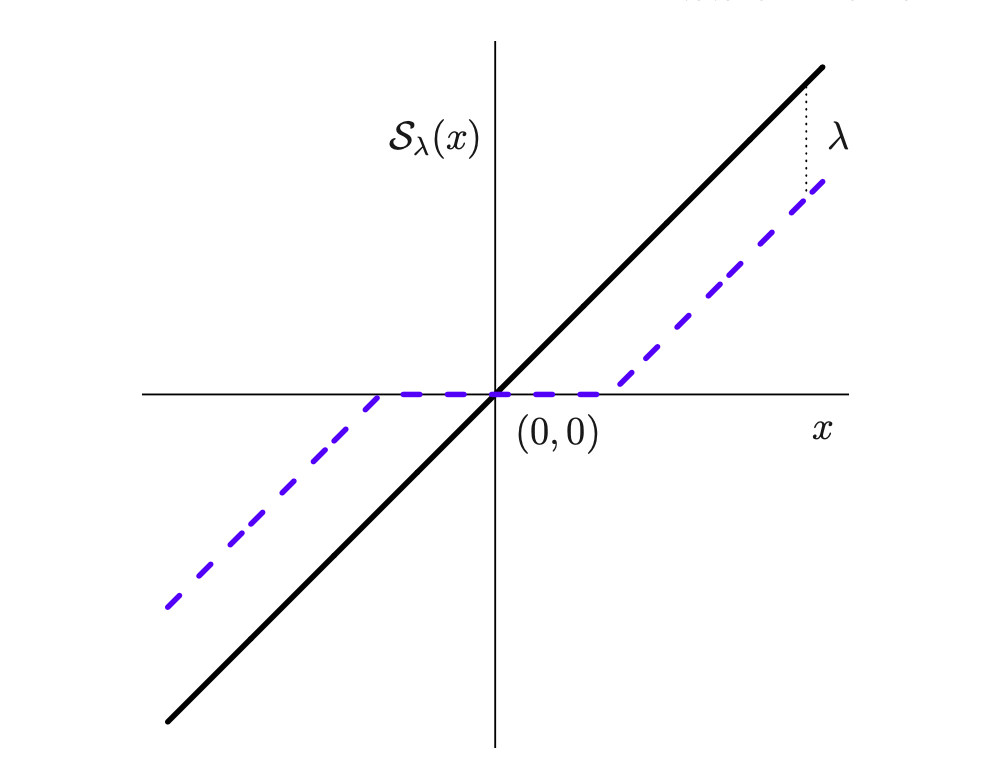
\includegraphics[scale=0.6]{soft_threshold}
  \caption[Soft thresholding function $S(x, \lambda)=\text{sign}(x)(|x|-\lambda)_+$]{
    Soft thresholding function $S(x, \lambda)=\text{sign}(x)(|x|-\lambda)_+$. The figure is from \cite{hastie2019statistical}. The blue broken line is the soft threshoding estimator, along with the $45^{\circ}$ line in black.
  }
  \label{fig:soft_threshold}
\end{figure}

There are some important properties of the lasso in addition to feature selection.
\begin{itemize}
    \item Just like ridge regression, the lasso also has an Bayesian interpretation. The prior distribution of $\bm{\beta}$ is double exponential/Laplace for the lasso, instead of normal for ridge.
    \item Degrees of freedom: Suppose there are $p$ features, fitting a linear regression using only a subset of $k$ of these features, if these $k$ features were chosen without regard to the outcome, the procedure spends $k$ degrees of freedom. However, if the $k$ features were chosen using knowledge of the outcome, for example best subset selection, then the fitting procedure spends more than $k$ degrees of freedom. Such a fitting strategy is adaptive, as well as the lasso. The lasso, with a fixed penalty parameter $\lambda$, the number of nonzero coefficients $k_\lambda$ is an unbiased estimate of the degrees of freedom \citep{zou2007degrees, tibshirani2012degrees}. The reason that lasso has exactly $k$ degrees of freedom rather than larger than $k$ is that it not only selects features which inflates the degrees of freedom, but also shrinks the coefficients. 
    \item The number of nonzero coefficients is at most $n$, the sample size, when the data is high dimensional, $p>n$.
    \item Assume that the underlying true signal is sparse, the lasso recovers the true signals well. If the underlying truth is not sparse, the lasso does not work well. 
\end{itemize}

\subsubsection{The elastic net}
Proposed by \cite{zou2005regularization}, the elastic net combines the ridge and the lasso; it solves the convex optimization problem
\begin{equation}
    \min_{\beta} \left\{ -\ell(\bm{\beta})+\lambda\left[\frac{1}{2}(1-c)\|\bm{\beta}\|_2^2+c\|\bm{\beta}\|_1\right] \label{eq1.10} \right\} 
\end{equation}
where $c\in [0,1]$ is a parameter that controls whether the penalty function to be more close to lasso or more close to ridge. When $c=1$, it reduces to $L_1$ norm, lasso penalty; when $c=0$, it reduces to squared $L_2$ norm, ridge penalty. The coordinate-wise update for the elastic net linear regression, again assuming the features are standardized to mean 0 and variance 1, is 
\begin{equation}
    \hat{\beta}_j^{enet} = \frac{S(\frac{1}{n}\sum_{i=1}^{n}x_{ij}r_i^{(j)}, \lambda c)}{1+\lambda(1-c)} \label{eq1.11}
\end{equation}
We can see the elastic net estimator shrinks the regression coefficients in the way of both lasso and ridge: it has the soft-thresholding portion truncating at $\lambda c$; it also shrink the coefficients proportionally with a factor of $1+\lambda(1-c)$. Hence, the elastic net shrinks the coefficients and some of them to exactly 0, so feature selection.

\subsection{Discussion of ridge regression, the lasso, the elastic net, and best subset selection}
\label{comparison_reg}
Best subset selection finds for each $k\in\{0,1,2,\dots,p\}$ the subset of size $k$ that gives smallest residual sum of squares (validation error). Best subset selection linear regression is equivalent to $L_0$ constrained regression, when design matrix $\bm{X}$ is orthogonal:
\begin{equation}
\begin{aligned}
    &\min_{\bm{\beta}} \frac{1}{2n}\|\bm{Y}-\bm{X\beta}\|_2^2, \\
    &\text{subject to} \quad \|\bm{\beta}\|_0 \leq k, \label{eq1.12}
\end{aligned}
\end{equation}
where $\|\bm{\beta}\|_0=\sum_{j=1}^p I(\beta_j \neq 0)$, is defined as the number of nonzero coefficients. Strictly speaking, $L_0$ is not a norm because it does not have properties of a norm, but the naming and notation are widely used. The $L_0$ constraint penalizes the number of nonzero coefficients, instead of the magnitude of coefficients. This exactly describes the best subset selection setting. And because it does not shrink the coefficients, the $L_0$ estimates are unbiased, while other regularization estimates are biased toward 0. Although, best subset selection, or $L_0$ constrained regression is superior in coefficient estimation, feature selection, it does not have an efficient algorithm, when $\bm{X}$ is not orthogonal. If we want to select a best subset without knowing how many features should be included to be the best subset, $k$, then there are $2^p$ combinations of features need to be examined. In other words, there are no polynomial time algorithm to solve it; the problem is NP-hard. Many approximation methods have been proposed to solve the problem. Among them, iterative hard thresholding is well performed. The closed form hard thresholding solution for $L_0$ constrained linear regression when $\bm{X}$ is orthogonal is   
\begin{equation}
    \hat{\bm{\beta}}^{L_0}=H_{\sqrt{2\lambda}}(\frac{1}{n}\bm{X}^T\bm{Y}), \label{eq1.13}
\end{equation}
where $H_{\sqrt{2\lambda}}(\cdot)$ is the hard thresholding operator,
\begin{equation}
    H_{\sqrt{2\lambda}}(\frac{1}{n}\bm{X}^T\bm{Y})=
    \begin{cases}
        \frac{1}{n}\bm{X}^T\bm{Y} & \text{if $|\frac{1}{n}\bm{X}^T\bm{Y}|>\sqrt{2\lambda}$}, \\
        0 & \text{if $|\frac{1}{n}\bm{X}^T\bm{Y}|\leq\sqrt{2\lambda}$}.
    \end{cases}
\end{equation}
It does not shrink regression coefficients at all, but truncates at $\sqrt{2\lambda}$. This is in close relation to the soft thresholding estimator of lasso, equation \eqref{eq1.9}, which shrinks coefficients by the amount of $\lambda$ and truncates at $\lambda$. This is why hard thresholding is an unbiased estimator of regression coefficient. In fact, the lasso is one of many approximations to $L_0$ constrained problem. And it is the closest convex approximation to it, while $L_0$ is a nonconvex optimization problem. Figure \ref{fig:estimators} shows the estimators for best subset/$L_0$, ridge, and lasso in the case of orthonormal orthogonal $\bm{X}$. We can see the unbiased estimator of best subset; feature selection ability of best subset and lasso; and different shrinkage scheme between ridge and lasso.
\begin{figure}[tbh]
  \centering
  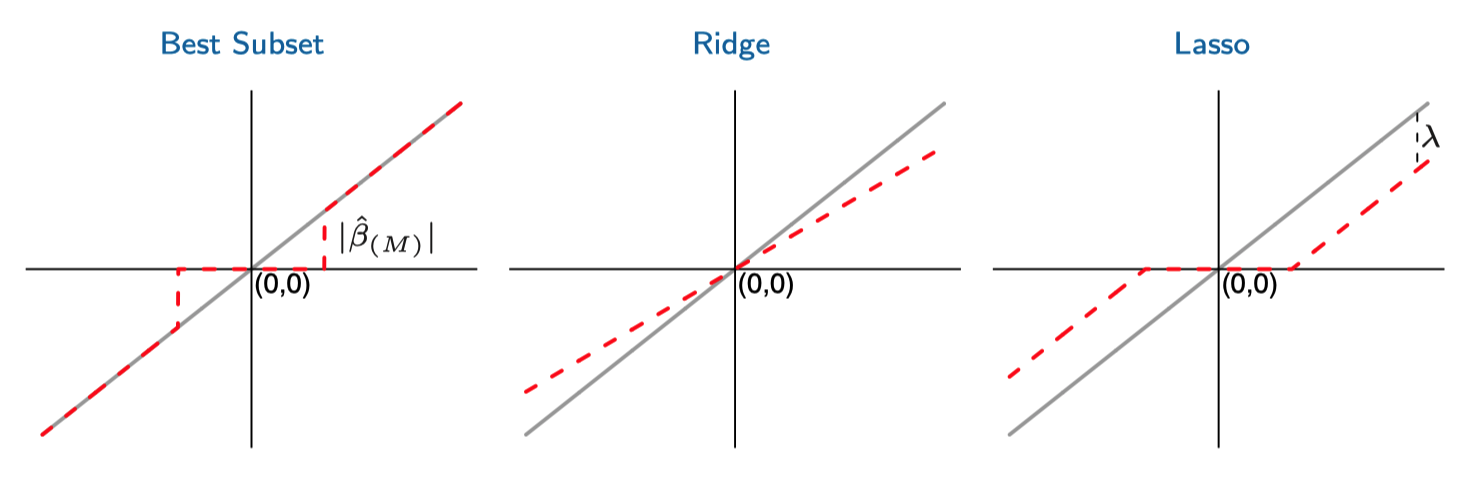
\includegraphics[scale=0.6]{estimator}
  \caption[Estimators of $\beta_j$ in the case of orthonormal columns of $\bm{X}$]{
    Estimators of $\beta_j$ for best subset, ridge, lasso, in the case of orthogonal column space of $\bm{X}$. Estimators are shown by broken red lines. The figure is from \cite{hastie2009elements}.
  }
  \label{fig:estimators}
\end{figure}

Ridge regression and the elastic net are also convex optimization problems. Since ridge, lasso and elastic net share this nice property, they have a highly efficient computational algorithm in pathwise coordinate descent \citep{friedman2007pathwise}. The algorithm solves the problems along a decreasing sequence of $\lambda$ values, for the purpose of tuning $\lambda$ via cross validation. Apart from giving a path of solutions, the algorithm exploits warm start, which initializes $\hat{\bm{\beta}}$ with the solutions of previous $\lambda$ value. This works because convex objective functions have continuous solutions along the path. By starting at previous solutions, coordinate descent updates need less iterations, thus leads to a more efficient and stable algorithm. On the other hand, iterative hard thresholding is not as efficient, and only guarantees to reach local minimums due to $L_0$'s nonconvexity. 

The lasso does not deal with highly correlated features very well; the solutions tend to be unstable. If there is a group of variables among which the pairwise correlations are very high, then the lasso tends to select only one variable randomly from the group. Ridge regression, on the other hand, shrink group correlated features toward each other. In other words, the features in a correlated group share the group effect evenly: having equal coefficients across the group and the coefficients add up to the group effect size. The elastic net is a combination of ridge and lasso. As we see the elastic net solution in equation \eqref{eq1.11}, it truncates the coefficients like lasso, shrink the coefficients proportionally like ridge. Therefore, it complements the inability of the lasso dealing with group correlated features with ridge regularization's grouping effect, which makes it a better choice when features are believed to have higher correlation structure.

\subsection{Nonconvex regularized regression} \label{sec:nonconvex}
Ridge regression, the lasso, the elastic net are all convex optimization problems. There are stable and efficient algorithms to solve it. And they always reach their global minimum solutions. Because of these, they are widely used for regularization, controlling model complexity. However, by moving from $L_2$ ridge to $L_1$ lasso, the shrinkage of some of the coefficients gets heavier, and finally being set to 0 when reach the lasso penalty. In fact, the lasso is the only convex regularization to produce sparse models. When the number of features is large and the true underlying model has only a few features, lasso is not able to shrink enough coefficients to 0. Nonconvex regularization leads to more sparse, less biased solutions. To see this, consider $L_q$ regularization,
\begin{equation}
    \min_{\bm{\beta}} \left\{ \frac{1}{2n}\|\bm{Y} - \bm{X\beta}\|_2^2 + \lambda \sum_{j=1}^{p}|\beta_j|^q \right\} \label{eq1.15}
\end{equation}
for $q\geq0$. It is the lasso for $q=1$, ridge for $q=2$. Figure \ref{fig:lq} displays $L_q$ regularization in the case of two inputs. For $0 \leq q <1$, the regularization is nonconvex, with the limiting $q=0$ corresponding to best subset selection. For these nonconvex constraints, they concentrate more mass in the coordinate directions, thus the solutions tend to be more sparse, and less shrinkage (biased toward 0). Unfortunately, along with nonconvexity comes combinatorial computational complexity and unstable algorithms. Alternative nonconvex regularization have been proposed.
\begin{figure}[tbh]
  \centering
  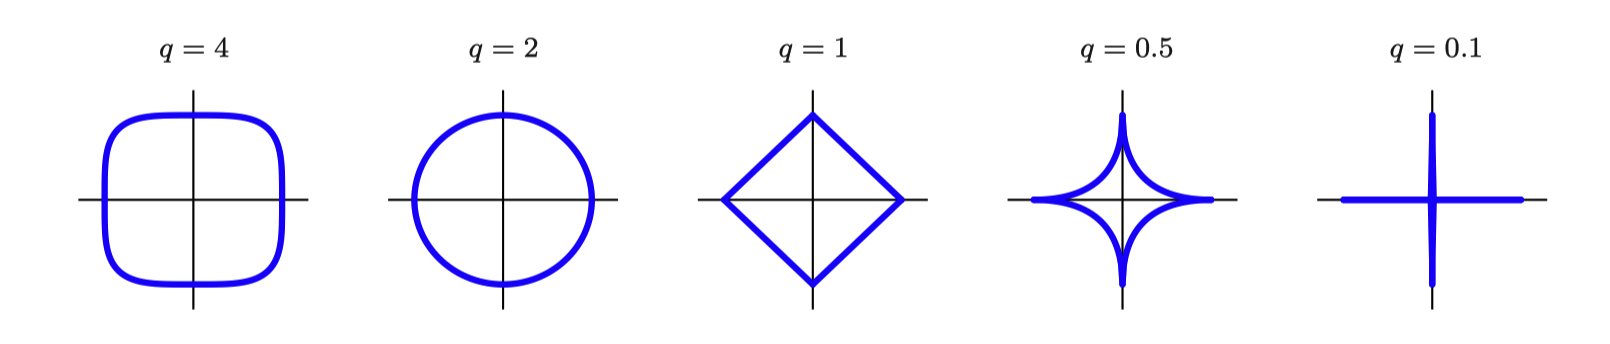
\includegraphics[width=\textwidth]{lq}
  \caption[Constraint regions $\sum_{j=1}^p|\beta_j|^q\leq1$ for different values of $q$] {
    Constraint regions $\sum_{j=1}^p|\beta_j|^q\leq1$ for different values of $q$. For $q<1$, the constraint region is nonconvex. The figure is from \cite{hastie2009elements}. 
  }
  \label{fig:lq}
\end{figure}

\subsubsection{Smoothed clipped absolute deviation penalty (SCAD) and minimax concave penalty (MCP)}
Proposed by \cite{fan2001variable}, the SCAD penalty defined on $[0, \infty)$ is given by (symmetric on $(-\infty, 0)$)
\begin{equation}
    P_{\lambda,\gamma}(\beta) = 
        \begin{cases}
            \lambda\beta & \text{if $\beta \leq \lambda$}\\
            \frac{\gamma\lambda\beta-0.5(\beta_2+\lambda^2)}{\gamma-1} & \text{if $\lambda<\beta\leq\gamma\lambda$}\\
            \frac{\lambda^2(\gamma^2-1)}{2(\gamma-1)} & \text{if $\beta>\gamma\lambda$}
        \end{cases} \label{eq1.16}      
\end{equation}
for $\lambda\geq0$ and $\gamma>2$. The univariate solution for a SCAD regularized simple linear regression coefficient is as follow
\begin{equation}
    \hat{\beta}=f_{SCAD}(z,\lambda,\gamma)= 
        \begin{cases}
            S(z,\lambda) & \text{if $|z|\leq 2\lambda$}\\
            \frac{S(z, \gamma\lambda/(\gamma-1))}{1-1/(\gamma-1)} & \text{if $2\lambda<|z|\leq\gamma\lambda$}\\
            z & \text{if $|z|>\gamma\lambda$}
        \end{cases} \label{eq1.17}      
\end{equation}
where $z=\frac{1}{n}\bm{X}^T\bm{Y}$ is the OLS solution.

Proposed by \cite{zhang2010nearly}, the MC+ penalty defined on $[0, \infty)$ is given by (symmetric on $(-\infty, 0)$)
\begin{equation}
    P_{\lambda,\gamma}(\beta) = 
        \begin{cases}
            \lambda\beta - \frac{\beta^2}{2\gamma} & \text{if $\beta \leq \gamma\lambda$}\\
            \frac{1}{2}\gamma\lambda^2 & \text{if $\beta>\gamma\lambda$}
        \end{cases} \label{eq1.18}      
\end{equation}
for $\lambda\geq0$ and $\gamma>1$. The univariate solution for a MC+ regularized simple linear regression coefficient is as follow
\begin{equation}
    \hat{\beta}=f_{MCP}(z,\lambda,\gamma)= 
        \begin{cases}
            \frac{S(z,\lambda)}{1-1/\gamma} & \text{if $|z|\leq \gamma\lambda$}\\
            z & \text{if $|z|>\gamma\lambda$}.
        \end{cases} \label{eq1.19}      
\end{equation}

The rational of SCAD and MCP is similar in that both penalties begin by applying same penalty as the lasso, and reduce the amount of penalty as the regression coefficient gets further away from zero. As a result of the penalty trend, when the coefficient is small in magnitude, it is shrunk to zero just like lasso; however, when the coefficient is large (larger than OLS solution), there is a transition region that shrinks the coefficient less than the lasso, and after the transition region, it is equal to the OLS solution without any shrinkage. This is a trend from less biased toward 0 to unbiased estimator, for those features with large effect sizes, thereby more likely to be associated with outcomes. Without the transition region, it is the hard thresholding estimator. The difference between SCAD and MCP is in the way they make transition. Figure \ref{fig:nonconvex_est} shows the trend of penalty functions of SCAD, MCP and their threshold functions. Indexed by nonconvexity parameter $\gamma$, it bridges the gap between lasso ($\gamma=\infty$) and best subset/hard threshold ($\gamma=2_+$ for SCAD, $1_+$ for MCP).   
\begin{figure}[tbh]
  \centering
  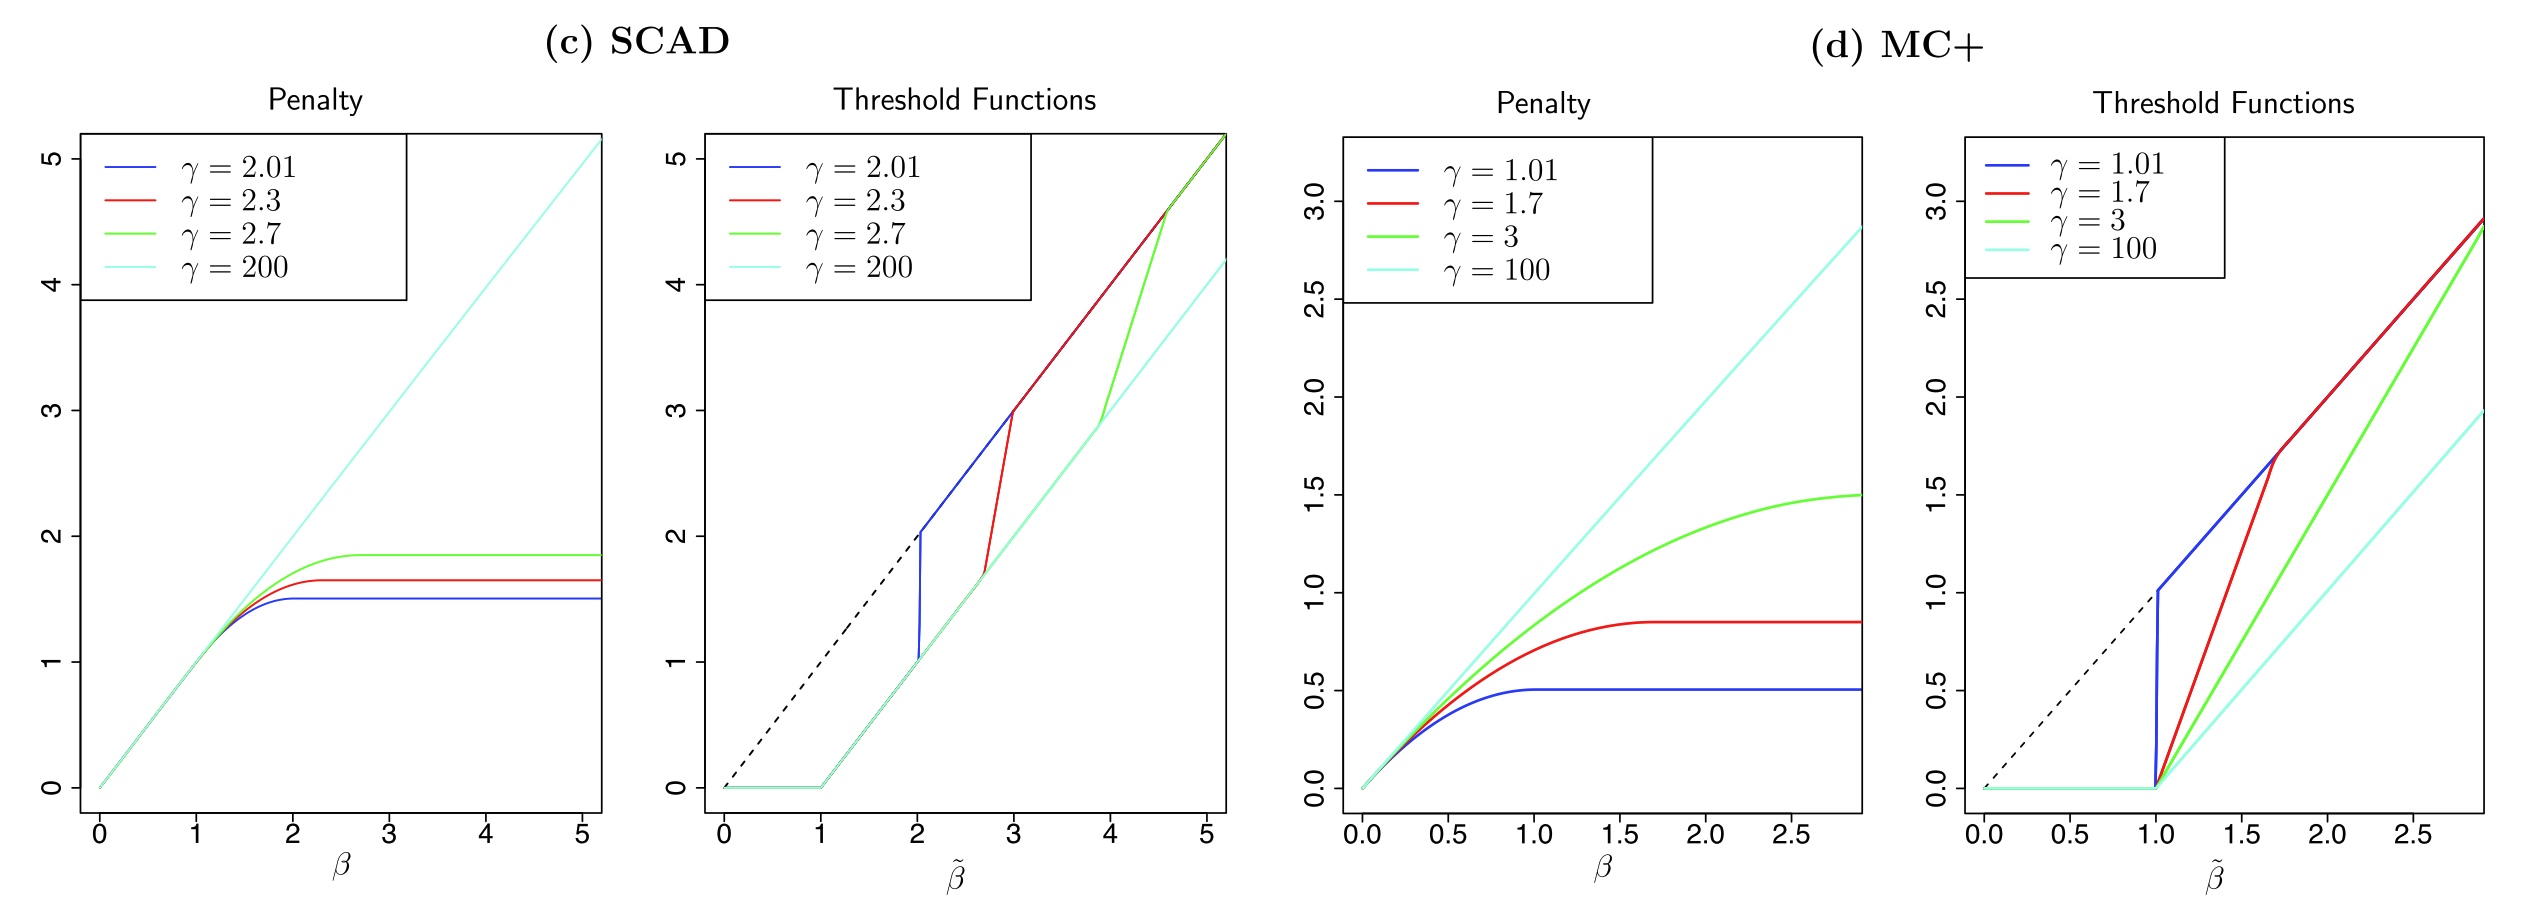
\includegraphics[width=\textwidth]{nonconvex_est}
  \caption[SCAD and MCP penalty functions and their corresponding threshold functions] {
    SCAD and MCP penalty functions and their corresponding threshold functions. Both are shown with $\lambda=1$ and different values for $\gamma$. The figure is from \cite{mazumder2011sparsenet}. 
  }
  \label{fig:nonconvex_est}
\end{figure}

The two nonconvex regularization techniques achieve less biased estimator, more sparse subset than the lasso. The choice of convex and nonconvex regularization depends on the application. For example, for a gene expression profile data, the underlying model is sparse but with a relatively large subset of features, the lasso is a better choice. Because with a large number of features in the model, say $1000-2000$, the direction of the feature coefficients are more meaningful rather than the magnitude of the coefficients. For a genetic association data, by which the underlying model only consists of a few markers, the accuracy of selection and unbiasedness of estimators are important. Hence, nonconvex regularization is a better suit in the situation.

We close the section by mentioning an approximation to $L_q$ ($0<q<1$) regularization that enjoys convex property.

\subsubsection{The adaptive lasso: approximation to nonconvex regularization}
Proposed by \cite{zou2006adaptive}, the adaptive lasso is a way of fitting models sparser than lasso. Using a pilot estimate $\tilde{\beta}$, the adaptive lasso has the form
\begin{equation}
    \min_{\bm{\beta}} \left\{ \frac{1}{2n}\|\bm{Y}-\bm{X\beta}\|_2^2+\lambda\sum_{j=1}^pw_j|\beta_j| \right\}, \label{eq1.20}
\end{equation}
where $w_j=1/|\tilde{\beta}_j|^v$. The adaptive lasso can be seen as an approximation to the $L_q$ regularization with $q=1-v$. We can see the adaptive lasso is convex in $\bm{\beta}$. Moreover, when the pilot estimates meet some regulatory conditions, the method recovers the true model under more general conditions than does the lasso. One can use least squares solution as the pilot estimate when $p<n$, univariate least squares solution when $p\geq n$. The indication is that, when least squares solution is small, the amount of penalty $w_j$ for feature $j$ is large, thereby $\hat{\beta}_j$ is more likely to be set to 0; when least squares solution is large, feature $j$ is penalized less (small $w_j$), then $\hat{\beta}_j$ is shrunk less, making it less likely to be 0 and less biased.

\section{Incorporating meta-features into modeling process}
As the types and the volume of genomics data are huge thanks to advanced high-throughput sequencing technologies, as well as the ever-growing annotation databases, there is increased need to integrate multiple types of genomics data, annotation data into modeling process. Because more related features provide more information to the outcome of interest, prediction performance can be improved. The traditional method is modeling one type of genomics data at a time, and combine the models in some form. As to utilizing annotation data, summary statistics, it is usually performed after modeling genomics data. This style of modeling different genomics data separately may ignore the interplay between them, the collective effect on the outcome. In this thesis, we introduced the concept meta-features, the features of the features. Now we introduce a second data matrix $\bm{Z}_{n\times p}$ that systematically stores extra data. Considering an annotation data that consists of several functional gene sets/pathways, and each gene set contains a group of genes. That is, if we have $p$ genomic features, $q$ functional gene sets (meta-features), the meta-feature matrix $\bm{Z}$ will have dimension $p\times q$, each row represents one genomic feature and has values of 0 or 1 indicating whether this genomic feature belongs to a gene set (1 indicates it belongs to the gene set, and 0 not). Table \ref{table:d1} shows the meta-feature matrix for gene sets.
\begin{table}[tbh]
    \centering
    \def\arraystretch{1.5}
    \begin{tabular}{|c|c|c|c|c}
        \hline
         & \textbf{gene set 1} & \textbf{gene set 2} & \textbf{gene set 3} & \dots \\ 
        \specialrule{.1em}{.05em}{.05em}
        gene 1 & 1 & 0 & 0 & \dots \\ 
        \hline
        gene 2 & 0 & 1 & 0 & \dots \\ 
        \hline
        gene 3 & 0 & 1 & 1 & \dots \\
        \hline
        \vdots & \vdots & \vdots & \vdots & $\ddots$ \\
    \end{tabular}
    \caption{Meta-feature matrix $\bm{Z}$ for gene sets/pathways}
    \label{table:d1}
    \end{table}

The usage of meta-feature matrix does not limit to annotation data, in fact, it can accommodate many types of information. We discuss 2 situations to show the flexibility of putting external data into meta-feature matrix $\bm{Z}$.

\begin{itemize}
    \item There are 3 types genomics data, gene expressions, single nucleotide polymorphisms (SNPs), DNA methylation  to be integrated into the modeling process. The meta-feature matrix tells which genomic feature is SNP, gene expression, or methylation. Table \ref{table:d2} shows the indicator meta-feature matrix. For example, ILMN\_343291 is a microarray probe, gene expression; rs10853372 is a SNP locus. 
    \begin{table}[tbh]
    \centering
    \def\arraystretch{1.5}
    \begin{tabular}{|c|c|c|c|}
        \hline
         & \textbf{Gene expression} & \textbf{SNP} & \textbf{Methylation} \\ 
        \specialrule{.1em}{.05em}{.05em}
        ILMN\_343291 & 1 & 0 & 0 \\ 
        \hline
        rs10853372 & 0 & 1 & 0 \\ 
        \hline
        ILMN\_1651210 & 1 & 0 & 0 \\
        \hline
        463100A3 & 0 & 0 & 1 \\
        \hline
        \vdots & \vdots & \vdots & \vdots \\
    \end{tabular}
    \caption{Meta-feature matrix $\bm{Z}$ for multiple types of genomics data}
    \label{table:d2}
    \end{table}
    
    \item There are summary statistics from similar studies on the same set of genomic features. These statistics from meta-analysis can be highly informative. They include p-values, hazard ratios, and source of features. In table \ref{table:d3}, gene BAX has a p\_value 0.0006 associated with the outcome, hazard ratio is 0.7605, the reason being included in the model is from previous GWAS studies. This is a hybrid matrix holding continuous values and indicator values: continuous values like p\-values, hazard ratios gives importance of the features; indicator variable tells the reason why the feature is included. 
    \begin{table}[tbh]
    \centering
    \def\arraystretch{1.5}
    \begin{tabular}{|c|c|c|c|c|c}
        \hline
         & \textbf{p\_value} & \textbf{Hazard ratio} & \textbf{Literature} & \textbf{GWAS}  \\ 
        \specialrule{.1em}{.05em}{.05em}
        BAX & 0.0006 & 0.7605 & 0 & 1 & \dots \\ 
        \hline
        IL6 & 0.2611 & -0.2077 & 1 & 0 & \dots \\ 
        \hline
        LDHB & $8.78\times 10^{-6}$ & 0.0768 & 0 & 1 & \dots \\
        \hline
        \vdots & \vdots & \vdots & \vdots & \vdots & $\ddots$ \\
    \end{tabular}
    \caption{Meta-feature matrix $\bm{Z}$ for summary statistics}
    \label{table:d3}
    \end{table}
\end{itemize}

With the above examples, we have shown the flexibility of the meta-feature matrix housing external information. Through the meta-feature matrix, we can integrate multiple types of genomics data, genomic annotation data, summary statistics from similar studies, and so on. It is the heart of our modeling process to integrate extra information that might be useful to prediction.

We propose two modeling strategy based on regularized regression. In chapter \ref{cha:xrnetcox}, we incorporate meta-features with a hierarchical structure
\[
\min_{\bm{\beta}} \left\{-\ell(\bm{\beta})+\frac{\lambda_1}{2}\|\bm{\beta}-\bm{Z\alpha}\|_2^2+\lambda_1\|\bm{\alpha}\|_1\right\},
\]
where $\ell(\bm{\beta})$ is log likelihood of regressing outcome on genomic features. And the coefficients of genomic features $\bm{\beta}$ are regressed on meta-features. This integrates meta-features linearly. In chapter \ref{cha:xtunecox}, we integrate meta-features in a non-linear way by allowing differential penalties for individual features, 
\begin{align*}
    &\min_{\bm{\beta}} \left\{-\ell(\bm{\beta}) + \sum_{j=1}^p \lambda_j\left[\frac{1}{2}(1-c)\beta_j^2 + c|\beta_j|\right]\right\}, \\
    &\lambda_j = e^{\bm{z_j}^T \bm{\alpha}}.
\end{align*}
The individualized penalty parameters $\lambda_j$'s are guided by meta-features, non-linearly with exponential function.
